\documentclass[iop]{emulateapj}
\usepackage{color}
\usepackage{natbib}
\bibliographystyle{apj}

\newcommand{\vdag}{(v)^\dagger}
\newcommand{\myemail}{eogorma@tcd.ie}

\shorttitle{Radio Emission of Dust-free Red Giant Mass Outflows}
\shortauthors{O'Gorman et al.}

\begin{document}

\title{Multi-frequency Radio Continuum Emission of Dust-free Red Giant Mass Outflows}


\author{Eamon O'Gorman\altaffilmark{1}, Graham M. Harper\altaffilmark{1}, Alexander Brown\altaffilmark{2}, Anita M.S. Richards\altaffilmark{3}, and Stephen Drake\altaffilmark{4}}
\altaffiltext{1}{School of Physics, Trinity College Dublin, Dublin 2, Ireland}
\altaffiltext{2}{Center for Astrophysics and Space Astronomy, University of Colorado, 389 UCB, Boulder, CO 80309, USA}
\altaffiltext{3}{Jodrell Bank Centre for Astrophysics, School of Physics and Astronomy, University of Manchester, Manchester M13 9PL, UK}
\altaffiltext{4}{NASA Goddard Space Flight Center, Greenbelt, MD 20771, USA}

%\email{eogorma@tcd.ie}
%\email{graham.harper@tcd.ie}
%\email{alexander.brown@colorado.edu}
%\email{a.m.s.richards@manchester.ac.uk}
%\email{drake@milkyway.gsfc.nasa.gov}

\begin{abstract}

Multi-frequency centimeter radio continumm observations of dust-free red giants directly sample their wind acceleration zones where most of the energy that drives their mass loss is being deposited. These stars are feeble thermal emitters at these wavelengths however, and previous observations have provided only a small number of modest signal-to-noise measurements accumulated over many years. Here, we present multi-frequency Karl G. Jansky Very Large Array (VLA) thermal continuum observations of the acceleration zones of two dust-free red giants, Arcturus and Aldebaran. Uniquely, these multi-frequency observations were mostly carried out within a few days of each other so any long term variability that may exist can be ignored. We report the first detections at many wavelengths for each star including a detection at 10 cm (3.0 GHz; S-band) for both stars and a 20 cm (1.5 GHz; L-band) detection for Arcturus. This is the first time single (non-binary) luminosity class III red giants have been observed at such long wavelengths. These measurements sample the outermost layers where the wind velocity is close to its terminal value and the ionization balance is close to becoming \textit{frozen-in}, and are therefore important empirical inputs for future wind models. We present spectral energy distributions for both stars and compare these with previous measurements and published semi-empirical models. The marked deviations between our data and existing semi-empirical models highlight the need for new atmospheric models to be developed.

\end{abstract}

\keywords{circumstellar matter --- Stars: individual: ($\rm{\alpha}$ Boo, $\rm{\alpha}$ Tau) --- Stars: late-type --- Stars: chromospheres --- Stars: winds, outflows --- Radio continuum: stars}

\section{INTRODUCTION}

Mass loss from late-type evolved stars plays a crucial role in both stellar and galactic evolution and ultimately provides part of of the material required for the next generation of stars and planets. Despite the importance of this phenomenon and decades of study, the mechanisms that drive winds from evolved spectral-type K through mid-M stars remain an enduring mystery (clearly laid out by \cite{1985ASSL..117..229H} but still unsolved, e.g.
\citealt{2009AIPC.1094..267C}). There is insufficient atomic, molecular, or dust opacity to drive a radiation-driven outflow and acoustic/pulsation models cannot drive the observed mass loss rates \citep{1995ApJ...442L..61S}. Optical and ultraviolet observations reveal an absence of hot wind plasma and the winds are thus too cool to be Parker-type thermally-driven flows \cite[e.g.][]{1979ApJ...229L..27L,1981ApJ...250..293A}. 

Magnetic fields are most likely involved in the mass loss process, although current magnetic models are also unsuccessful. Exquisite high signal-to-noise (S/N) ratio \textit{Hubble} ultraviolet (UV) spectra have revealed that the 1-D linear Alfv\'en wave-driven wind models of the 1980’s (e.g., \citealt{1980ApJ...242..260H}) are untenable. These models predict chromospheres as integral parts of turbulently extended and heated wind acceleration zones, but the theoretical line profiles and electron densities do not agree with the \textit{Hubble} spectra, e.g., \cite{1998ApJ...494..828J}. One important property of cool evolved star winds gleaned from UV spectra is that, for the most part, the red giant winds accelerate in a quasi-steady manner and are not the result of ballistic ejecta. A new generation of theoretical models with outflows driven within diverging magnetic flux tubes have now emerged \citep{2006MNRAS.368.1145F, 2007ApJ...659.1592S} but these too are not currently in agreement with observations \citep{2009AIPC.1094..267C}. It has also been suggested that the winds may be driven by some form of magnetic pressure acting on highly clumped wind material \citep{2008AJ....136.1964E} but \cite{2010ApJ...720.1767H} does not find support for this hypothesis. Progress in this field continues to be driven by observations that provide new insights into the mass loss problem.

\subsection{Radio Continuum Observations} \label{intro1} 

Although studies of wind-scattered UV and optical line profiles have provided clues to the mass-loss rates and radial distribution of the mean and turbulent velocity fields, the thermal structure remains poorly constrained. In the UV, the source function is very sensitive to electron temperature (i.e. $S_{\nu} \propto e^{-h\nu /kT}$) and so a localized hot plasma component in a dynamic atmosphere can completely dominate the temporally and spatially averaged emission and not reflect the global mean value. At radio wavelengths however, the source function is thermal and is just the Rayleigh-Jeans tail of the Planck function, which is linear in electron temperature (i.e. $S_{\nu} = {2kT\nu ^2 /c^2}$) and so should give a more appropriate estimate of the thermal radial wind structure. It is this value that controls the atomic level populations and ionization that feed into UV spectroscopic analyses. This value is also needed to quantify the implied thermal heating supplied to the  wind by the unknown driving source/sources, and thus derive constraints on potential mass loss mechanisms.

In the cm-radio regime the radio opacity strongly increases with wavelength (i.e. $ \kappa \propto \lambda ^{2.1}$) so the longer wavelengths sample the extended layers of the stars atmosphere thus essentially providing us with spatial information about the star's mass outflow region. The thermodynamic properties in this spatial region control the ionization in the far wind because the ionization balance, which also controls the cooling rates, becomes frozen-in at these radii. Furthermore, it is these outer extended regions of the star's atmosphere that contribute to the commonly seen P Cygni line profiles in the UV. In these profiles the line-of-sight absorption caused by the star's wind is superimposed on the blueshifted emission. Thus, centimeter radio continuum observations can provide a test of models based on these UV profiles. In this paper we directly compare our new Karl G. Jansky Very Large Array (VLA) observations with atmospheric models derived from UV analysis.

\subsection{Sample Selection} \label{intro2}

Currently the most detailed spatial information about the atmospheres of K and early M evolved stars is obtained from eclipsing binaries such as the symbiotic and $\zeta$ Aurigae systems (e.g. \citealt{2008ApJ...675..711C};   \citealt{1996ApJ...466..979B}). Even though these systems offer us the best opportunity to obtain information on the dynamics and thermodynamics at various heights in the evolved star's atmosphere, the very nature of the binary system may introduce further complexities. For example, the orbital separation is often within the wind acceleration region and one could expect wind accretion and flow perturbations to be present (e.g. \citealt{1981ApJ...248.1043C}). In fact, using the ``old'' VLA, \cite{2005AJ....129.1018H} confirm that the velocity structure of  of $\zeta$ Aurigae is not typical of single stars with similar spectral types. 

In order to avoid the assumed additional complexities of a companion, we have selected two single luminosity class III red giants: Arcturus ($\alpha$ Boo: K2 III) and Aldebaren ($\alpha$ Tau: K5 III). These nearby red giants have been extensively studied at other wavelengths and their stellar parameters, which are briefly summarized in Table 1, are accurately known. These stars are predicted to be point sources at all frequencies in all VLA configurations so our radio observations measure their total flux density. Moreover both stars have existing semi-empirical 1-D chromospheric and wind models which we directly test the validity of in this paper. 

\begin{deluxetable}{ccc}
\tabletypesize{\scriptsize}
\tablecaption{Some properties of our red giant sample.}
\tablehead{	\colhead{}		       				& 
			\colhead{$\alpha$ Boo}				&
			\colhead{$\alpha$ Tau}				}
\startdata
Spectral Type 				& K2 III  & K5 III  \\
Effective Temperature (K)	& $4294 \pm 30$  & $3970 \pm 49$ \\
Angular Diameter (mas)		& $21.0 \pm 0.2$ & $20.2 \pm 0.3$ \\
Wind Temperature (K)		& $\sim 10,000$  & $< 10,000$  \\
Wind Terminal Velocity & $\sim$ 40 km s$^{-1}$ & $\sim$ 30 km s$^{-1}$ \\
Semi-empirical model	& \cite{1985pssl.proc..351D} & \cite{1999MNRAS.302...37M}
\enddata
\tablecomments{Effective temperatures and photospheric diameters are taken from \cite{1993AA...270..315D}.}

\label{tab:tab1}
\end{deluxetable}

\begin{deluxetable*}{ccccccccc}
\tabletypesize{\scriptsize}
%\tablecolumns{6} 
%\tablewidth{0pt} 
\tablecaption{VLA Observations}
\tablehead{\colhead{Star}			            &
\colhead{Date}
				&
          	\colhead{Band}	      				&
          	\colhead{Frequency\tablenotemark{a}}&
	\colhead{Wavelength}			         	&
           	\colhead{Time on Star}              &
           	\colhead{Bandwidth}            		&
           	\colhead{Number of}            		&
	\colhead{Phase}		\\
	\colhead{}									&
    \colhead{}		                			& 
    \colhead{}		                			& 
	\colhead{(GHz)}                        		& 
	\colhead{(cm)}                         		& 
	\colhead{(hr)}                    			&
	\colhead{(GHz)}                        		&
	\colhead{Antennas\tablenotemark{b}}         &
	\colhead{Calibrator}		}
\startdata
$\alpha$ Boo	& 2011 Feb 22 & Q	& 43.3 & 0.7		& 0.3 	&  0.256	&22& J1357+1919  \\
$\alpha$ Boo 	& 2011 Feb 22 & Ka	& 33.6 & 0.9		& 0.2 	&  0.256 	&23&J1357+1919  \\
$\alpha$ Boo 	& 2011 Feb 22 & K	& 22.5 & 1.3		& 0.4	&  0.256 	&24&J1357+1919  \\
$\alpha$ Boo 	& 2011 Feb 11 & X	& 8.5  & 3.5		& 0.3 	&  0.256 	&18&J1415+1320  \\
$\alpha$ Boo	& 2011 Feb 11 & C	& 5.0  & 6.0 		& 0.5	& 0.256 	&21& J1415+1320 \\
$\alpha$ Boo	& 2011 Feb 13 & S	& 3.1  & 9.5 		& 1.8 	& 0.256 	&12& J1415+1320 \\
$\alpha$ Boo 	& 2012 Jul 19 & S	& 3.0  & 10.0 		& 0.7 	& 2.0 		&23& J1415+1320 \\
$\alpha$ Boo	& 2012 Jul 20 & L	& 1.5  & 20.0		& 1.6 	& 1.0 		&23& J1415+1320 \\
$\alpha$ Tau	& 2011 Feb 11 & Q	& 43.3 & 0.7 		& 0.3 	& 0.256 	&22&  J0431+1731\\
$\alpha$ Tau	& 2011 Feb 11 & Ka	& 33.6 & 0.9 		& 0.2 	& 0.256 	&19&  J0449+1121\\
$\alpha$ Tau	& 2011 Feb 11 & K	& 22.5 & 1.3 		& 0.4 	& 0.256 	&21&  J0449+1121\\
$\alpha$ Tau	& 2011 Feb 13 & X	&  8.5 & 3.5 		& 0.5	& 0.256 	&25&  J0449+1121\\
$\alpha$ Tau	& 2011 Feb 13 & C	&  5.0 & 6.0 		& 1.2	& 0.256 	&21&  J0449+1121\\
$\alpha$ Tau	& 2011 Feb 12 & S	&  3.1 & 9.5 		& 1.8 	& 0.256 	&11&  J0431+2037
\enddata
\tablenotetext{a}{Central frequency of used bandpass.}
\tablenotetext{b}{Number of available antennas remaining after flagging.}
\label{tab:tab2}
\end{deluxetable*}


\section{OBSERVATIONS AND DATA REDUCTION}

Observations of $\alpha$ Boo and $\alpha$ Tau were carried out with the VLA during February 2011 at Q, Ka, K, X, C, and S-band in B-configuration (PI: Harper; program 10C-105). $\alpha$ Boo was also observed at S and L-band in July 2012 when the VLA was again in B-configuration (PI: O'Gorman; program 12A-472). Some details of these observations are given in Table \ref{tab:tab2}. For the 2011 observations, the correlator was set up with two 128 MHz sub-bands centered on the frequencies listed in Table \ref{tab:tab2}. Each sub-band had sixty-four channels of width 2 MHz and four polarization products (RR, LL, RL, LR). For the S and L band observations in 2012, the 1-2 GHz and 2-4 GHz frequency ranges were both divided into 16 sub-bands, each with sixty-four channels. The channel width was 2 and 1 MHz for S and L-band, respectively.

Both $\alpha$ Boo and $\alpha$ Tau were slightly offset from the phase-center by $\sim$\,5 synthesized beam widths in order to avoid possible errors at phase-center. All scheduling blocks (SBs) were kept to $\le$\,2.5 hours of duration to improve their likelihood of being scheduled. For the high frequency observations (i.e. Q, Ka, and K-bands) we used the \textit{fast switching} technique which consisted of rapidly alternating observations of the target source and a nearby unresolved phase calibrator. The total cycle times for the Q, Ka, and K-band observations were 160, 230, and 290 s, respectively. For both target sources these high frequency observations were combined into a single 2 hour observing track and commenced with X-band reference pointing with solutions being applied on-line. After X-band pointing the target source was observed at Q-band to insure the best pointing solutions were used. The lower frequencies tracks were composed of repeatedly interleaving observations of the target source and a nearby phase calibrator but had much longer cycle times. The primary calibration sources 3C286 and 3C138 were observed at the end of all tracks and were used to measure the complex bandpass and set the absolute flux for $\alpha$ Boo and $\alpha$ Tau, respectively.  

The data were flagged, calibrated, and imaged within the Common Astronomical Software Application  \cite[CASA;][]{2007ASPC..376..127M} package. Data deemed to be bad by the VLA online system were flagged, as were pure zeros, non-operational antennas antennas, dummy scans at the beginning of each track, and poorly performing antennas. Visual inspection of each scan was carried out to determine if data at the beginning or end of these scans needed to be flagged (a process known as \textit{quacking}). For the 2011 low frequency data the two sub-bands were centered at relatively radio frequency interference (RFI) free regions of the bandpass and only a very small amount of RFI had to be flagged.   The 2012 wide-band data was initially Hanning smoothed (combining adjacent frequency channels with weights 0.25, 0.5, and 0.25) to suppress Gibbs ringing. We manually flagged entire sub-bands that were badly contaminated with RFI. The \textit{testautoflag} task was then used to conservatively flag RFI from all sources and any remaining RFI was manually flagged. 

In order to calibrate the data, we solved for the complex gains of the calibration sources while applying the bandpass solution, which was derived from the relevant aforementioned flux calibrators.  The amplitude gains of the phase calibrators were scaled according to values derived from the flux calibrators using the ``Perley-Butler 2010" flux density standard. At the time, no Ka or S-band flux density standard models were available so instead for these we used the K and L-band models, respectively. The more frequently observed phase calibrators were then used to calibrate the amplitude and phases of the targets. Atmospheric opacity corrections were also applied to the high frequency data sets using the average of a seasonal model (based on many years of measurements) and information from the weather station obtained during the observations.

The visibilities were then both Fourier transformed and deconvolved using the CASA \textit{clean} task in multi-frequency synthesis imaging mode, which separately grids the the multiple spectral channels onto the \textit{u-v} plane and therefore improves the overall \textit{u-v} coverage. We used natural weighting for maximum sensitivity and the cell size was chosen so that the synthesized beam was about five pixels across. For the high frequencies it was usually sufficient to place just one CLEAN circle around the target source.  For the low frequencies however, the image sizes were usually set to a few times the size of the primary beam so that nearby strong serendipitous sources could be CLEANed thus reducing their sidelobe contamination of the final image. These images were CLEANed interactively, with w-term correction, down to about the $3\sigma$  level with clean boxes placed around sources as they appeared in the residual image. All images were corrected for  primary beam attenuation. 

Three different methods were used to calculate the flux density from the unresolved target sources in each image:
\begin{enumerate}
\item by taking the peak pixel value from the source
\item by manually integrating the flux density around the source
\item by fitting an elliptical Gaussian model to the source and deriving the integrated flux density using the CASA \textit{imfit} task.
\end{enumerate}
Each of these values along with the image root mean square (rms) noise measured from adjacent background regions and fitting error produced by \textit{imfit} are given in Table \ref{tab:tab3}. We assume absolute flux density scale systematic uncertainties of  3\% at all frequencies.

\begin{deluxetable*}{Cccccccc}
\tabletypesize{\scriptsize}
%\tablecolumns{6} 
%\tablewidth{0pt} 
\tablecaption{VLA Fluxes of $\alpha$ Boo and $\alpha$ Tau}
\tablehead{\colhead{}		            &
			\colhead{Band}		            &
			\colhead{Frequency\tablenotemark{a}}&
			\colhead{Peak Flux}					&
          	\colhead{Integrated Flux} 			&
          	\colhead{\textit{Imfit} Integrated}	&
			\colhead{Image rms}					&
           	\colhead{\textit{Imfit} Fitting}  	\\
	\colhead{}									&
	\colhead{}									&
	\colhead{(GHz)}								&
    \colhead{(mJy)}		        	& 
    \colhead{(mJy)}		                		& 
	\colhead{Flux (mJy)}                        		& 
	\colhead{(Jy beam^{-1})}         					&
	\colhead{Error (mJy)}		}
\startdata
$\alpha$ Boo (K2 III) &Q  &43.28& 5.941 & 6.093 & 6.420 & 0.301 &  0.261\\
&Ka &33.56& 4.159 & 4.319 & 4.489 & 0.083 & 0.090 \\
&K  &22.46& 1.827 & 1.784 & 1.809 & 0.043 & 0.050 \\
&X  &8.46 & 0.510 & 0.514 & 0.532 & 0.030 & 0.019 \\
&C  &4.90 & 0.214 & 0.144 & 0.159 & 0.035 & 0.009 \\
&S  &3.15 & 0.148 & 0.135 & 0.160 & 0.028 & 0.010\\
&S  &2.87 & 0.127 & 0.118 & 0.116 & 0.012 & 0.016\\
&L  &1.63 & 0.067 & 0.068 & 0.090 & 0.013 & 0.015\\
\hline
\rule{0pt}{3ex}  $\alpha$ Tau (K5 III)&Q  &43.28 & 3.672& 3.734 & 4.082 &  0.259& 0.183	\\
&Ka &33.56 & 2.188& 1.962 & 2.125 &  0.091& 0.070 \\
&K  &22.46 & 1.864& 1.881 & 2.069 &  0.042& 0.083 \\
&X  &8.46  & 0.296& 0.287 & 0.281 &  0.014& 0.015 \\
&C  &4.96  & 0.147& 0.167 & 0.176 &  0.010& 0.010 \\
&S  &3.15  & 0.062& 0.043 & - &  0.017 & -
\enddata
\tablenotetext{a}{Frequency of final image produced using \textit{clean}'s multi-frequency synthesis imaging mode.}
\label{tab:tab3}
\end{deluxetable*}

\section{RESULTS} 

Apart from $\alpha$ Boo at C-band and $\alpha$ Tau at S-band, detections were made in both sub-bands for the 2011 data. The flux densities of the targets in both sub-bands were found to be the same within their uncertainties so we do not present these values here. Instead we give the values from the radio maps produced by concatenating the two sub-bands. We present in Table \ref{tab:tab3} the target flux densities extracted from these concatenated radio maps. In the following two sections we briefly discuss the properties of these radio maps for both targets.

\subsection{$\alpha$ Boo Radio Maps} \label{results1} 
High S/N detections ($>19\sigma$) of $\alpha$ Boo were made at 22.5, 33.6, and 43.3 GHz. Some residuals of the dirty beam remained in the CLEANed maps due to the paucity of uv-coverage in these short high frequency observations. The lower frequencies maps were contaminated by the emission of a strong radio source located $186\arcsec$ north-west of $\alpha$ Boo. This source was reported by \cite{1986AJ.....91..602D} and their flux of 25 mJy at 4.9 GHz is in close agreement with our measurement of 23.2 mJy at the same frequency. We find the source to have a spectral index of -1.4 and its flux reaches  80.3 mJy at 1.6 GHz. Surprisingly we do not detect $\alpha$ Boo in the higher frequency sub-band at 5.0 GHz (C-band) so the values given in Table \ref{tab:tab3} are taken from the lower frequency sub-band only. We obtain good detections ($>5\sigma$) of the star for both epochs at 3 GHz (S-band) and the peak flux densities agree within their uncertainties. We can therefore safely assume that the 1.5 GHz (L-band) flux has not changed significantly over that period either, and so can safely be included in any analysis. The map at L-band was highly contaminated by the emission of the strong source north-west of $\alpha$ Boo but the star is still detected at the $5\sigma$ level. There is a slight positional offset of $1\arcsec$ between the position of the peak flux for $\alpha$ Boo at 1.5 and 3.0 GHz for the 2012 data, which were taken within 1 day of each other. However, this is less than a quarter of the 1.5 GHz synthesized beam and considering that the $4\sigma$ contours overlap, we feel that it is highly unlikely that both sources are not $\alpha$ Boo. 

\subsection{$\alpha$ Tau Radio Maps} \label{results2}
The final deconvolved radio maps of $\alpha$ Tau were of excellent quality with the rms noise reaching the predicted thermal noise in many cases. The target field at all frequencies was free from strong serendipitous radio sources and thus the final images were free of the sidelobe contamination that were present in the low frequency $\alpha$ Boo images. $\alpha$ Tau was the only source in the high frequency maps while the brightest source in the low frequency maps was located $106\arcsec$ north north-east of $\alpha$ Tau and had a flux of 0.85, 1.35, and 1.7 mJy at 8.5, 5.0, and 3.5 GHz, respectively. Strong detections ($>14\sigma$) of $\alpha$ Tau were made at all frequencies between 5.0 and 43.3 GHz. Due to the limited number of S-band receivers installed at the time, a full 2.5 hr track was dedicated to $\alpha$ Tau at 3.1 GHz in order to achieve the required sensitivity to give a possible detection. We report a tentative $3\sigma$ detection of $\alpha$ Tau at 3.1 GHz when we take its peak pixel value as its total flux density. As this is a weak detection we avoid using the \textit{imfit} task to obtain a flux density estimate, as this may introduce further errors \citep{1999ASPC..180.....T}.

\begin{deluxetable*}{Ccccc}
\tabletypesize{\scriptsize}
%\tablecolumns{6} 
%\tablewidth{0pt} 
\tablecaption{Compilation of Previous $\alpha$ Boo and $\alpha$ Tau Observations ($\le 250$ GHz)}
\tablehead{							            &
    \colhead{Frequency}		       				& 
			\colhead{Date}						&
			\colhead{Flux Density}				&
          	\colhead{Source} 			\\
												&
	\colhead{(GHz)}								&
	\colhead{}									&
    \colhead{(mJy)}		        				& 
    \colhead{}			         				}
\startdata
$\alpha$ Boo (K2 III) &4.9  & 1983 Jan 21 & $0.39 \pm 0.13$ & \cite{1986AJ.....91..602D} \\
&4.9  & 1983 May 20 & $0.26 \pm 0.08$ & \cite{1986AJ.....91..602D} \\
&4.9  & 1983 Dec 26 & $\le 0.18(3\sigma)$ & \cite{1986AJ.....91..602D} \\
&4.9  & 1984 Mar 17 & $0.24 \pm 0.05$ & \cite{1986AJ.....91..602D} \\
&15 & 1984 Nov 6 & $0.68 \pm 0.09$ & \cite{1986AJ.....91..602D} \\
&22.5  & 1999 Jan 06  & $ 1.7 \pm 0.2$ & \cite{2011AA...533A.107D} \\
&43.3  & 1999 Jan 06 & $ 3.3 \pm 0.4$ & \cite{2011AA...533A.107D} \\
&43.3  & 2004 Jan 25 & $ 3.34 \pm 0.08$ & \cite{2011AA...533A.107D} \\
&86  & 1985 Nov  & $ 21.4 \pm 7.5$ & \cite{1986AA...164..227A} \\
&108.4  & 1997 Nov - 2000 Jun & $ 20.09 \pm 0.69$ & \cite{2005AJ....129.2836C} \\
&217.8 & 1997 Nov - 2000 Jun  & $ 83.5 \pm 1.71$ & \cite{2005AJ....129.2836C} \\
&250  & 1986 Dec - 1989 Mar  & $ 78 \pm 8$ & \cite{1994AA...281..161A} \\
\hline
\rule{0pt}{3ex}    $\alpha$ Tau (K5 III)	&4.9  & 1983 Jan 21 & $\le 0.27(3\sigma)$ & \cite{1986AJ.....91..602D} \\
&4.9  & 1984 Nov 6 & $\le 0.22(3\sigma)$ & \cite{1986AJ.....91..602D} \\
&5.0  & 1997 Sep 27 & $\le 0.07(3\sigma)$		& Brown \& Harper (private communication) \\
&8.5  & 1997 Sep 27 & $0.28 \pm 0.03$ 		& Brown \& Harper (private communication) \\
&14.9 & 1997 Sep 27 & $0.95 \pm 0.08$ 		& Brown \& Harper (private communication) \\
&15 & 1984 Nov 6 & $0.60 \pm 0.1$ 		& \cite{1986AJ.....91..602D} \\
&108.4  & 1997 Nov - 2000 Dec & $ 13.97 \pm 1.46$ & \cite{2005AJ....129.2836C} \\
&217.82 & 1999 Sep - 2000 Dec  & $ 25.78 \pm 5.64$ & \cite{2005AJ....129.2836C} \\
&250  & 1986 Dec - 1987 Jan & $ 51 \pm 6$ & \cite{1994AA...281..161A} 
\enddata
\label{tab:tab4}
\end{deluxetable*}

\section{DISCUSSION}
\subsection{Spectral Energy Distribution of $\alpha$ Boo} \label{disc1}
The first definite detection of a single red giant at centimeter wavelengths was of $\beta$ Gem by \cite{1983ApJ...274L..77D}. Included in this study was a probable $3\sigma$ detection of $\alpha$ Boo and since then there has been only a small number of sporadic centimeter and millimeter observations of the star. In Table \ref{tab:tab3} we list the majority of these observations and plot their flux densities as a function of frequency in Figure \ref{fig:fig1}. We also include in this figure the chromosphere and wind models of \cite{1985pssl.proc..351D} which were based on the International Ultraviolet Explorer (IUE) Mg II k emission line and the overlap between the two models are represented by the green shaded area. At high frequencies the models predict the slope of the spectral energy distribution to be blackbody-like (i.e. $\sim \nu ^{2}$) as a result of the small density scale heights close to the star. At low frequencies however, the models predict the wind to have constant velocity, ionization and temperature and thus the slope  approaches the well known $\sim \nu ^{0.6}$ limit \citep{1975MNRAS.170...41W,1975AA....39..217O,1975AA....39....1P}. The paucity and, in some cases low S/N, of previous observations make it difficult to discern the validity of this model prior to our multi-frequency study of this star.

The peak flux density values listed in Table \ref{tab:tab3} for $\alpha$ Boo are also included in Figure \ref{fig:fig1} along with their $1\sigma$ rms errors. Our new data reveal significant deviations from the current existing semi-empirical model at both low and high frequencies (in this case below $\sim$ 8 GHz and above $\sim$ 25 GHz). At low frequencies this discrepancy may indicate that we are still sampling a region of the wind where it is still accelerating (i.e. it has not yet reached its terminal velocity) or may also be a manifestation of rapid wind cooling further out than that predicted in UV spectral analysis. Our highest frequency data points indicate a flux excess which is in agreement with previous higher frequency (i.e. mm-observations) observations. One notable exception to this high frequency flux excess are the two 43 GHz observations of \cite{2011AA...533A.107D} which are lower than our values by over 40\%. Such a level of chromospheric viability seems very high and would be unexpected from such supposedly inactive stars. Another possibility for the difference in values  is that the longer cycle times used by \cite{2011AA...533A.107D}, which was over double our value, may cause larger phase errors and thus lower final flux density values. Future high frequency observations may clarify this matter.


\subsection{Spectral Energy Distribution of $\alpha$ Tau} \label{disc2}
\\
d
\\
\\
zz
\\
\\
\\
\\
d
\\
\\
zz
\\
\\
\\
\\
d
\\
\\
zz
\\
\\
\\
\subsection{Contribution Functions?} \label{disc3}
\subsection{Mass loss e.g. Drake & Linskey ?} \label{disc4}
\subsection{Future Atmospheric Models e.g. Advection?} \label{disc5}

\begin{figure*}
\centering
\includegraphics[trim = 0mm 0mm 0mm 20mm, clip,scale=0.65, angle=90]{fig1.ps}
\\
\caption{Spectral energy distribution of $\alpha$ Boo for frequencies less than 250 GHz. Our new multi-frequency VLA observations which were mainly acquired over a few days in February 2011 are the blue circular data points and appear to be in disagreement with the existing chromospheric and wind models of \cite{1985pssl.proc..351D} which are shown in green. The red circular data points are all of the previous observations which were acquired sporadically over the past $\sim 25$ years.}
\label{fig:fig1}
\centering
\includegraphics[trim = 0mm 0mm 0mm 20mm, clip,scale=0.65, angle=90]{fig2.ps}
\\
\caption{Spectral energy distribution of $\alpha$ Tau for frequencies less than 250 GHz. All our new $\alpha$ Tau multi-frequency VLA observations (blue circular data points) were acquired in just two days in February 2011. The red circular data points are all of the previous observations which were acquired over many years. The green line is an existing hybrid chromosphere and wind model for the star.}
\label{fig:fig2}
\end{figure*}

\section{CONCLUSIONS}

\acknowledgments
The data presented in this paper were obtained with the Karl G. Jansky Very Large Array (VLA) which is an instrument of the National Radio Astronomy Observatory (NRAO). The NRAO is a facility of the National Science Foundation operated under cooperative agreement by Associated Universities, Inc. We wish to thank the NRAO helpdesk for their detailed responses to our CASA related queries.

{\it Facilities:} \facility{VLA}.

\bibliography{references}

\end{document}